\documentclass{beamer}

% does not look nice, try deleting the line with the fontenc.
\usepackage[english]{babel}
\usepackage{amsmath}
\usepackage[latin1]{inputenc}
\usepackage{units}
\usepackage{colortbl}
\usepackage{multimedia}
\usepackage{bm}
\usepackage{subcaption}
\usepackage{algorithm2e}
\usepackage{algorithmic}

\mode<presentation>
{
  \usetheme{Boadilla}
  \useoutertheme{infolines}
  \setbeamercovered{transparent} 
}
	

\title[Dynamical systems \& deep learning]{{Deep learning with transfer functions: New applications in system identification}}


\author[]{Dario Piga, \underline{Marco Forgione}, Manas Mejari}

\institute[IDSIA]{IDSIA Dalle Molle Institute for Artificial Intelligence USI-SUPSI, Lugano, Switzerland} 


\date[]{19th IFAC symposium System Identification: learning models for decision and control}


\subject{System Identification, Deep Learning, Machine Learning, Regularization}


%% MATH DEFINITIONS %%
\newcommand{\So}{S_o} % true system
\newcommand{\hidden}[1]{\overline{#1}}
\newcommand{\nsamp}{N}
\newcommand{\Yid}{Y}
\newcommand{\Uid}{U}
\newcommand{\Did}{{\mathcal{D}}}
\newcommand{\tens}[1]{\bm{#1}}

\newcommand{\batchsize}{q}
\newcommand{\seqlen}{m}
\newcommand{\nin}{n_u} 
\newcommand{\ny}{n_y} 
\newcommand{\nx}{n_x}

\newcommand{\NN}{\mathcal{N}} % a feedforward neural network

\newcommand{\norm}[1]{\left \lVert #1 \right \rVert}
\DeclareMathOperator*\argmin{arg \, min}
\newcommand{\Name}{\emph{dynoNet}}


%% DYNONET MATH DEFINITIONS %%
\newcommand{\q}{q} % shift operator
\newcommand{\A}{A} % autoregressive polynomial
\newcommand{\ac}{a} % autoregressive polynomial coefficient
\newcommand{\B}{B} % exogenous polynomial
\newcommand{\bb}{b} % exogenous polynomial coefficient
\newcommand{\Gmat}{\mathbb{G}} % transfer function operator in matrix form
\newcommand{\tvec}[1]{\bm{#1}}
\newcommand{\mat}[1]{\bm{#1}}
\newcommand{\sens}[1]{\tilde{#1}}
\newcommand{\adjoint}[1]{\overline{#1}}
\newcommand{\loss}{\mathcal{L}}
\newcommand{\pdiff}[2]{\frac{\partial #1}{\partial #2}}
%\newcommand{\nsamp}{T}

\newcommand{\conv}{*}
\newcommand{\ccorr}{\star}
\definecolor{orange}{RGB}{204, 85, 0}
%% DYNONET %%

\definecolor{darkgreen}{RGB}{20,150,50}
\definecolor{Periwinkle}{rgb}{0.0, 0.0, 0.0}
\usepackage{listings}
\newcommand{\book}{\includegraphics[width=10pt]{img/proceeding-logo.jpg}}
\newcommand{\github}{\includegraphics[width=10pt]{img/github-logo.jpg}}
\begin{document}

\begin{frame}
  \titlepage
\end{frame}


\begin{frame}{Motivations}
Two main classes of \structure{neural network} structures for system identification:
\begin{columns}
\column{.48\textwidth}
\begin{block}{Recurrent NNs}
 General state-space models
 \vskip 1em
    \begin{itemize}
     \item High representational capacity
     \item Hard to parallelize
     \item Numerical issues in training
    \end{itemize}
 \end{block}
\column{.48\textwidth}
\begin{block}{1D Convolutional NNs}
  Dynamics through FIR blocks
  \vskip 1em
    \begin{itemize}
     \item Lower capacity, several params
     \item Fully parallelizable
     \item Well-posed training
    \end{itemize}
\end{block}
\end{columns}

\pause
\vskip 2em
We have recentily introduced \Name\,: an architecture using linear
\structure{transfer functions} as  building blocks.
%\pause

\begin{itemize}
	\item[\book]
		\begin{tiny}
	\structure{M.~Forgione and D.~Piga.}
									\emph{dynoNet}: A Neural Network architecture for learning dynamical systems.
									\vskip -1em
									\emph{International Journal of Adaptive Control and Signal Processing}, 2021
		\end{tiny}\\								
% 	\item[\book]
% 		\begin{tiny}
% 	\structure{D.~Piga, M.~Forgione and M.~Mejari.}
% 									Deep learning with transfer functions: new applications in system identification.
% 									\vskip -1em
% 									\emph{Accepted to the 2021 SysId Conference (Invited session ``Linear identification and control for nonlinear systems'')}, 2021
% 		\end{tiny}\\								
\end{itemize}
\end{frame}


\begin{frame}{The \Name\ architecture}{}%{dynoNet}
Deep learning with the LTI \structure{transfer functions}.
 \begin{columns}[t]
  \column{.45\textwidth}
    \begin{figure}
        \centering
        A feed-forward neural network
        \vskip 1em
        \includegraphics[width=\textwidth]{img/dynonet/FCNN.pdf}
    \end{figure}  
 \column{.1\textwidth}
 \begin{center}
 \vskip 5em
 $\Rightarrow$
 \end{center}
 \column{.45\textwidth}
    \begin{figure}
        \centering
        A dynoNet
        \vskip 2em
        \includegraphics[width=\textwidth]{img/dynonet/generic_dynonet.pdf}
    \end{figure}  
 \end{columns}
 \vskip 1.5em
\begin{itemize}
 \item An extension of feed-forward neural networks, with dynamical blocks
 \item An extension of 1D CNNs, with Infinite Impulse Response dynamics
 \item An extension of block-oriented models, with arbitrary connections
\end{itemize}
\end{frame}

\begin{frame}{Related works}
\structure{Block-oriented} architectures extensively studied in System Identification. Interconnection of transfer functions $G(z)$ and static non-linearities $F(\cdot)$:
\begin{columns}
\column{.2\textwidth}
 \begin{figure}
 \footnotesize Wiener
 \vskip .5em
 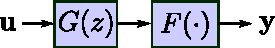
\includegraphics[width=\textwidth]{img/dynonet/wiener.pdf}
 \end{figure}
\column{.2\textwidth}
 \begin{figure}
 \footnotesize Hammerstein
 \vskip .5em
 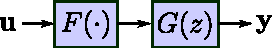
\includegraphics[width=\textwidth]{img/dynonet/hammer.pdf}
 \end{figure}
 \column{.3\textwidth}
 \begin{figure}
 \footnotesize Wiener-Hammerstein
 \vskip .5em
 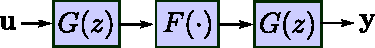
\includegraphics[width=\textwidth]{img/dynonet/wiener_hammerstein.pdf}
 \end{figure}
\end{columns}
\vskip 0em
%shallow architectures, SISO blocks \dots
\begin{columns}
\column{.4\textwidth}
 \begin{figure}
	 \footnotesize Generalized Hammerstein-Wiener
 \vskip .5em
 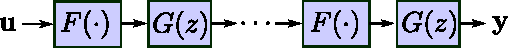
\includegraphics[width=\textwidth]{img/dynonet/generalized_HW.pdf}
 \end{figure}
 \column{.4\textwidth}
 \begin{figure}
 \vskip 1em
 \footnotesize Parallel Wiener-Hammerstein
 \vskip 1em
 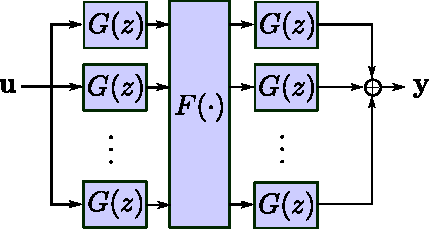
\includegraphics[width=.9\textwidth]{img/dynonet/parallel_WH.pdf}
 \end{figure}
\end{columns}
\vskip 1em
%\pause
%Training with \structure{specialized algorithms} requiring, e.g., {analytic} expressions of gradients/jacobians.
 \end{frame}

 \begin{frame}{Related works}
\begin{itemize}
 \item  \Name\ generalizes block-oriented models to \structure{arbitrary connection} of MIMO blocks $G(z)$ and $F(\cdot)$
 \item More importantly, training is performed using a \structure{general approach} 
 \item Plain \structure{back-propagation} for gradient computation exploiting deep learning software
\end{itemize}
\begin{figure}
 \vskip 0em
 \footnotesize a \Name\ network
 \vskip .5em
 \includegraphics[width=.60\textwidth]{img/dynonet/generic_layer.pdf}
\end{figure}
\pause
\alert{Technical challenge}: back-propagation through the transfer function! \\
No hint in the literature, no ready-made implementation available.
\end{frame}

\begin{frame}{Transfer function}

Transforms an input sequence $u(t)$ to an output $y(t)$ according to:
\begin{footnotesize}
	$$y(t) = G(\q)u(t) = \frac{B(\q)}{A(\q)} = \frac{\bb_0 + \bb_1 \q^{-1} + \dots + \bb_{n_{\bb}}q^{-n_{\bb}}}{1 + \ac_1 \q^{-1} + \dots + \ac_{n_\ac}q^{-n_\ac}} u(t)$$
\end{footnotesize}
Equivalent to the recurrence equation:
\begin{footnotesize}
$$ y(t) = \bb_0 u(t) + \bb_1 u(t-1) + \dots + \bb_{n_\bb}\!u(t-n_\bb)-\ac_1 y(t\!-\!1) \dots - \ac_{n_\ac} y(t\!-\!n_\ac).$$
\end{footnotesize}
%\end{equation}

\pause

For our purposes, $G$ is a \structure{vector operator} with coefficients $a$, $b$, transforming $\tvec{u} \in \mathbb{R}^\nsamp$ to $\tvec{y} \in \mathbb{R}^\nsamp$
%\begin{footnotesize}
$$
 \tvec{y} = G(\tvec{u}; a, b)
$$
%\end{footnotesize}
\pause
%\vskip .5em
Our goal is to provide $G$ with a \structure{back-propagation} behavior.\\
The operation has to be \structure{efficient}!
\end{frame}

\begin{frame}{Forward pass}
In back-propagation-based training, the user defines a \structure{computational graph} producing a \structure{loss} $\loss$ (to be minimized). \\


\vskip 2em
In the \structure{forward pass}, the loss $\loss$ is computed.\\
$G$ receives $\tvec{u}$, $a$, and $b$ and needs to compute $\tvec{y}$:
\begin{columns}
\column{.5\textwidth}
$$
 \tvec{y} = G.\mathrm{forward}(\tvec{u}; a, b).
$$
\column{.5\textwidth}
\begin{figure}
\includegraphics[width=.8\textwidth]{img/dynonet/forward_tf_ab.pdf}
\end{figure}
\end{columns}

\pause
\vskip 2em
The forward pass for $G$ is easy: it is just the linear recurrence equation: \\
\begin{footnotesize}
$$ y(t) = \bb_0 u(t) + \bb_1 u(t-1) + \dots + \bb_{n_\bb}\!u(t-n_\bb)-\ac_1 y(t\!-\!1) \dots - \ac_{n_\ac} y(t\!-\!n_\ac).$$
\end{footnotesize}
\vskip .5em
Computational cost: \color{darkgreen}{$\mathcal{O}(N)$}.
\end{frame}

 \begin{frame}{Backward pass}
 \begin{itemize}
 \item In the \structure{backward pass}, derivatives of $\loss$ w.r.t. the \structure{training variables} are computed. 
 Notation:  $\adjoint{x} = \pdiff{\loss}{x}$. 
 \item The procedure starts from $\adjoint{\loss} \equiv \pdiff{\loss}{\loss} = 1$ and goes \structure{backward}.
 \item Each operator must be able to ``push back'' derivatives from its outputs to its inputs
 \end{itemize}
 \vskip 1em

\uncover<2->{
 $G$ receives $\adjoint{\tvec{y}} \equiv \pdiff{\loss}{\tvec{y}}$ and is responsible for computing:
 $\adjoint{\tvec{u}}, \adjoint{a}, \adjoint{b}$:
 \begin{columns}
 \column{.5\textwidth}
 $$
  \adjoint{\tvec{u}}, \adjoint{a}, \adjoint{b} = G.\mathrm{backward}(\adjoint{\tvec{y}}; a, b).
 $$
 \column{.5\textwidth}
 \only<1>{
 \begin{figure}
 \includegraphics[width=.8\textwidth]{img/dynonet/backprop_tf_ab_empty.pdf}
 \end{figure}
 }
 \only<2->{
 \begin{figure}
 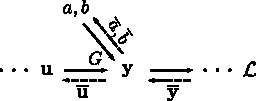
\includegraphics[width=.8\textwidth]{img/dynonet/backprop_tf_ab.pdf}
 \end{figure}
 }

 \end{columns}
}
 \vskip 1.5em 
\uncover<3->{
 The \structure{chain rule} is the basic tool, but certain tricks may be used to \structure{speed up} the operation. Computational cost also {\color{darkgreen}{$\mathcal{O}(N)$}}, all details in the  paper\dots \\
}
 \end{frame}


\begin{frame}[fragile]{PyTorch implementation}
%PyTorch implementation of the differentiable transfer function %in the repository \url{https://github.com/forgi86/dynonet}.
 \begin{itemize}
  \item[\github]\begin{tiny}{\url{https://github.com/forgi86/dynonet}}\end{tiny}
  \item[\github]\begin{tiny}{\url{https://github.com/forgi86/sysid-transfer-functions-pytorch}}\end{tiny}
  \end{itemize}

\vskip 1em
\centering
Use case:
\vskip .2em
\begin{columns}
 \column{.5\textwidth}
 \begin{center}
 \vskip -.5em
 \Name \ architecture
\begin{figure}
 \vskip 0em
 \includegraphics[width=.8\textwidth]{img/dynonet/specific_dynonet.pdf}
\end{figure}
\end{center}
\column{.5\textwidth}
 \begin{center}
 %\vskip -.1em
 Python code
  \begin{tiny}
\begin{lstlisting}[language=python]


G1 = LinearMimo(1,  4, ...) # a SIMO tf
F = StaticNonLin(4, 3, ...) # a static NN
G2 = LinearMimo(3, 1, ...) # a MISO tf
G3 = LinearMimo(1, 1, ...) # a SISO tf
 
def model(in_data):  
    y1 = G1(in_data)
    z1 = F(y1) 
    y2 = G2(z1)
    out = y2 + G3(in_data)
    
\end{lstlisting}
\end{tiny}
\end{center}
\end{columns}
 \vskip 1em 
 \pause
 \begin{flushleft}
 Any \structure{gradient-based} optimization algorithm can be used to train the \Name. The derivatives are obtained through \structure{back-propagation}.
 \end{flushleft}

\end{frame}

\begin{frame}{Experimental results}
  On \structure{public benchmarks} at \url{www.nonlinearbenchmark.org}.\\
  
  \begin{center}
   Wiener-Hammerstein System
  \end{center}

  \begin{columns}
   \column{.33\textwidth}
    \centering
   \begin{figure}
   \footnotesize
    \includegraphics[height=.3\textheight]{img/dynonet/WH_circuit.png}
    \end{figure}
  \column{.33\textwidth}
      \begin{figure}
 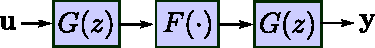
\includegraphics[height=.1\textwidth]{img/dynonet/wiener_hammerstein.pdf}
    \end{figure}
   \column{.33\textwidth}
    \centering
   \begin{figure}
   \footnotesize
    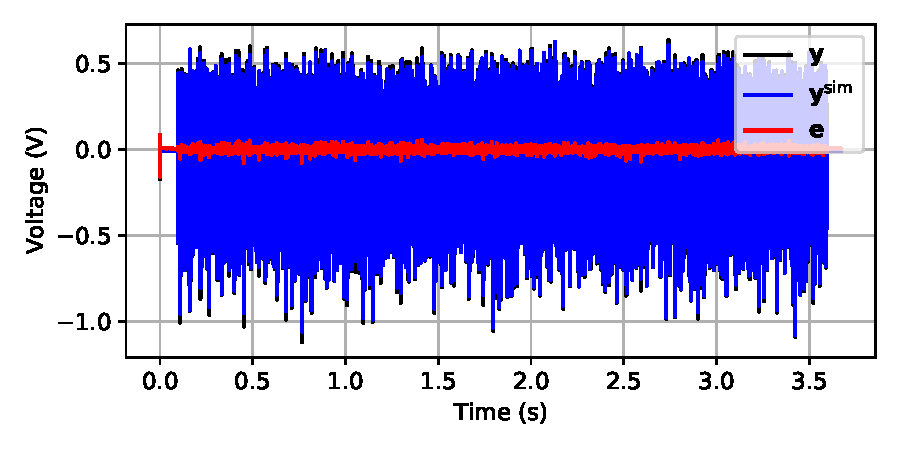
\includegraphics[height=.3\textheight]{img/dynonet/WH_timetrace.pdf}
   \end{figure}
  \end{columns}
  
  \vskip 4em
  %\centering
  Test performance: $\mathrm{fit} = 99.5\%$\\
\end{frame}
  
  
\begin{frame}{Experimental results}
  On \structure{public benchmarks} at \url{www.nonlinearbenchmark.org}.\\
  
  \begin{center}
   Parallel Wiener-Hammerstein
  \end{center}

  \begin{columns}
   \column{.33\textwidth}
    \centering
   \begin{figure}
   \footnotesize
    \includegraphics[height=.1\textheight]{img/dynonet/PWH_benchmark.png}
    \end{figure}
  \column{.33\textwidth}
      \begin{figure}
 \includegraphics[height=.25\textwidth]{img/dynonet/parallel_WH_benchmark.pdf}
    \end{figure}
   \column{.33\textwidth}
    \centering
   \begin{figure}
   \footnotesize
    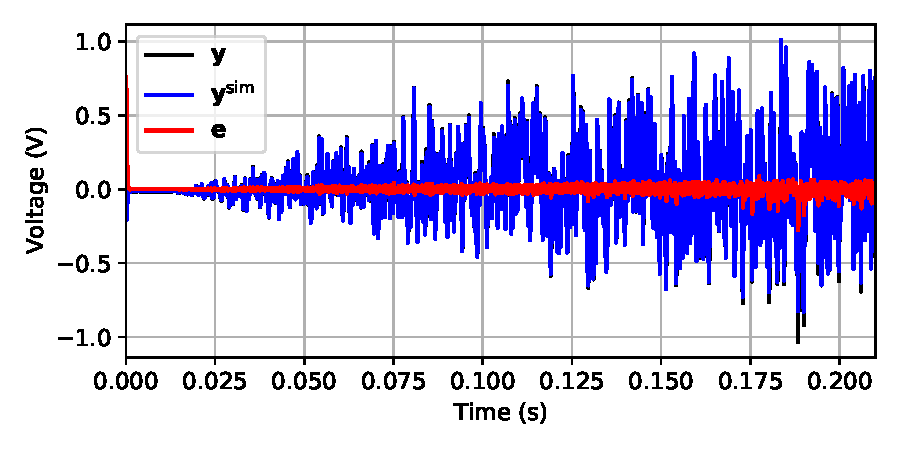
\includegraphics[height=.3\textheight]{img/dynonet/PWH_timetrace.pdf}
   \end{figure}
  \end{columns}
  
  \vskip 4em
  %\centering
  Test performance: $\mathrm{fit} = 98.4\%$\\
  \end{frame}
   
\begin{frame}{Experimental results}
  On \structure{public benchmarks} at \url{www.nonlinearbenchmark.org}.\\
  
  \begin{center}
   Bouc-Wen Hysteretic System
  \end{center}

  \begin{columns}
   \column{.33\textwidth}
    \centering
   \begin{figure}
    \includegraphics[height=.3\textheight]{img/dynonet/BW_hyst.png}
    \end{figure}
      \column{.33\textwidth}
%      \begin{figure}
\includegraphics[height=.15\textheight]{img/dynonet/generic_dynonet.pdf}
%    \end{figure}

   \column{.33\textwidth}
    \centering
   \begin{figure}
    \includegraphics[height=.3\textheight]{img/dynonet/BW_timetrace.pdf}
   \end{figure}
  \end{columns}
  \vskip 2em
  Test performance: $\mathrm{fit} = 93.2\%$\\
  \end{frame}
  

\begin{frame}{Experimental results}
  On \structure{public benchmarks} at \url{www.nonlinearbenchmark.org}.\\
  
  \begin{center}
   Wiener-Hammerstein System\\
   modified training dataset, additive \structure{colored noise} on the output 
  \end{center}

  \begin{columns}
   \column{.33\textwidth}
    \centering
   \begin{figure}
   \footnotesize
    \includegraphics[height=.3\textheight]{img/dynonet/WH_circuit.png}
    \end{figure}
  \column{.33\textwidth}
      \begin{figure}
 %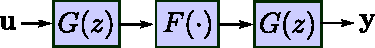
\includegraphics[height=.1\textwidth]{img/dynonet/wiener_hammerstein.pdf}
 %\vskip 1em
 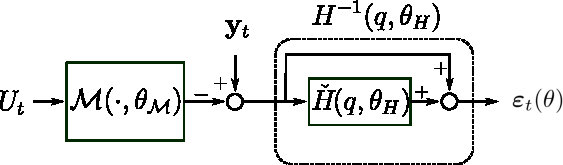
\includegraphics[height=.3\textwidth]{img/dynonet/neural_PEM.pdf}

 \end{figure}
   \column{.33\textwidth}
    \centering
   \begin{figure}
   \footnotesize
    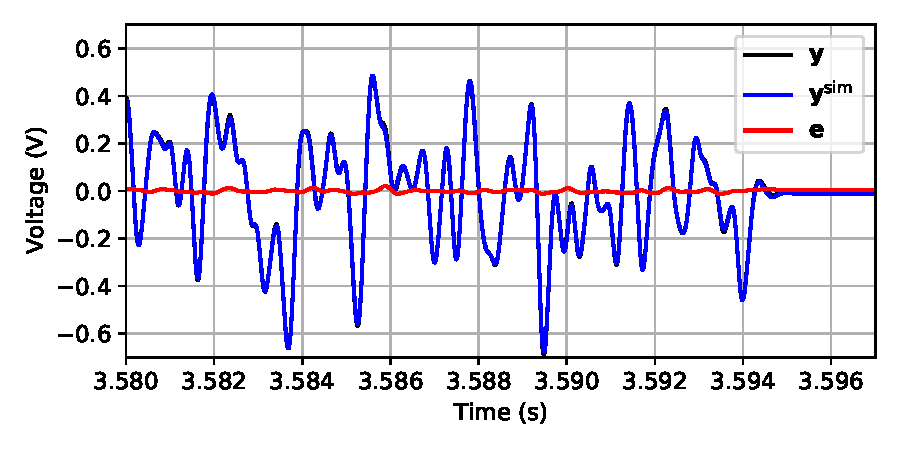
\includegraphics[height=.2\textheight]{img/dynonet/WH_timetrace_zoom.pdf}
    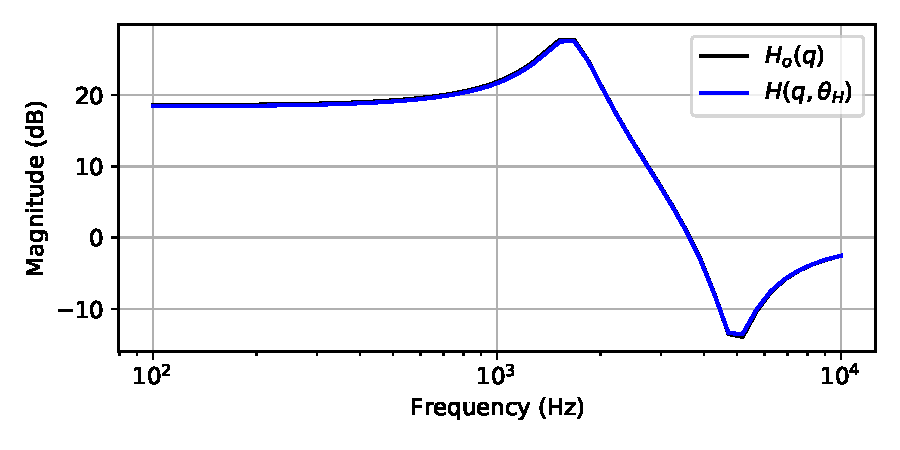
\includegraphics[height=.2\textheight]{img/dynonet/WH_H.pdf}
   \end{figure}
  \end{columns}
  
  \vskip 2em
  %\centering
  Training with WH model + noise whitening filter (Neural PEM)\\
  Test performance: $\mathrm{fit} = 96.9\%$\\
  \end{frame}

   \begin{frame}{Experimental results}
  On \structure{public benchmarks} at \url{www.nonlinearbenchmark.org}.\\
   \begin{center}
   Parallel Wiener-Hammerstein\\
   modified training dataset, 5-level quantized measurements 
  \end{center}

  \begin{columns}
   \column{.33\textwidth}
    \centering
   \begin{figure}
   \footnotesize
    \includegraphics[height=.08\textheight]{img/dynonet/parallel_WH_quant.png}
    \end{figure}
  \column{.33\textwidth}
      \begin{figure}
 %\includegraphics[height=.25\textwidth]{img/dynonet/parallel_WH_benchmark.pdf}
 %\vskip 1em
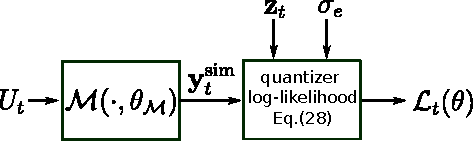
\includegraphics[height=.25\textwidth]{img/dynonet/dynonet_quant.pdf}
 \end{figure}
   \column{.33\textwidth}
    \centering
   \begin{figure}
   \footnotesize
    \includegraphics[height=.3\textheight]{img/dynonet/PWH_quant_timetrace.pdf}
   \end{figure}
\end{columns}
  
  \vskip 4em
  %\centering
  Training with a loss corresponding to ML for quantized measurements:\\
  Test performance: $\mathrm{fit} = 91.9\%$\\

  \end{frame}

\begin{frame}{Conclusions}
A neural network architecture containing linear dynamical operators parametrized as 
 rational transfer functions.
 \vskip 1em
 \begin{itemize}
  \item Extends \structure{1D-Convolutional} NNs  and \structure{block-oriented} models%to Infinite Impulse Response dynamics
  %\item Extends  with arbitrary interconnections
  \item Training through \structure{plain back-propagation}, at cost $\mathcal{O}(N)$\\ 
  %No custom algorithm/code required
  \item Implementation available on-line
%  \item New applications: neural PEM and quantized measurements
 \end{itemize}
\vskip 1em
%We obtained good performance on public identification benchmark.
\pause
Current and future work:
\begin{itemize}
 \item Estimation/control strategies
 \item System analysis/model reduction using e.g. linear system tools 
\end{itemize}

\end{frame}

\begin{frame}{}{}
\begin{center}
\huge{\structure{Thank you.\\ Questions?}}\\
\vskip 1em
\begin{small}
\texttt{marco.forgione@idsia.ch}
\end{small}
\end{center}
\end{frame}

\appendix

 \begin{frame}{Backward pass for $\tvec{u}$}
 
 Compute $\adjoint{\tvec{u}} \equiv \pdiff{\loss}{\tvec{u}}$ from $\adjoint{\tvec{y}}\equiv \pdiff{\loss}{\tvec{y}}$. \\
 \pause
 \begin{itemize}
 \item Applying the chain rule:
 \begin{footnotesize}
$$\adjoint{\tvec{u}}_\tau = \pdiff{\loss}{\tvec{u}_\tau} 
= \sum_{t=0}^{\nsamp-1}{\pdiff{\loss}{\tvec{y}_t} \pdiff{\tvec{y}_t}{\tvec{u}_\tau}}
=\sum_{t=0}^{\nsamp-1}{\adjoint{\tvec{y}}_t \tvec{g}_{t-\tau}}
$$
\end{footnotesize}
where $\tvec{g}$ is the \structure{impulse response} of $G$.%contains the impulse response coefficients
\pause
\item From the expression above, by definition:
\begin{footnotesize}
$$\adjoint{\tvec{u}} = \tvec{g} \ccorr \adjoint{\tvec{y}},
$$
\end{footnotesize}
where  $\ccorr$ is \structure{cross-correlation}.
This implementation has cost  \alert{$\mathcal{O}(\nsamp^2)$}
\pause
\item It is equivalent to filtering $\adjoint{\tvec{y}}$ through $G$ in reverse time, and flipping the result. Implemented this way, the cost is {\color{darkgreen}{$\mathcal{O}(\nsamp)$}}! 
$$ \adjoint{\tvec{u}} = \mathrm{flip}\big(G(q) \mathrm{flip}(\adjoint{\tvec{y}})\big)$$
\pause  All details (also for $\adjoint{a}$ and $\adjoint{b}$) in the paper\dots
\end{itemize}
\end{frame}


 \begin{frame}{Backward pass for $b$}
 
 Compute $\adjoint{b} \equiv \pdiff{\loss}{b}$ from $\adjoint{\tvec{y}}\equiv \pdiff{\loss}{\tvec{y}}$. \\
 \pause
 \begin{itemize}
 \item Applying the chain rule:
 \begin{footnotesize}
$$\adjoint{b}_j = \pdiff{\loss}{b_j} 
= \sum_{t=0}^{\nsamp-1}{\pdiff{\loss}{\tvec{y}_t} \pdiff{\tvec{y}_t}{b_j}}
%=\sum_{t=0}^{\nsamp-1}{\adjoint{\tvec{y}}_t \tvec{g}_{t-\tau}}
$$
\end{footnotesize}
\pause
\item The \structure{forward sensitivities}  $\pdiff{\tvec{y}_t}{b_j}$ may be obtained in closed form through additional filtering 
operations. From the definition:
\begin{footnotesize}
\begin{align*}
 A(q) y(t) &= B(q) u(t)\\
 y(t) + \ac_1 y(t\!-\!1) \dots + \ac_{n_\ac} y(t\!-\!n_\ac) &= \bb_0 u(t) + \bb_1 u(t-1) + \dots + \bb_{n_\bb}\!u(t-n_\bb)\\
\end{align*}
%\end{footnotesize}
\pause
\vskip -3em
Differentiating w.r.t. $b_j$:
%\begin{footnotesize}
\begin{align*}
 \pdiff{y(t)}{b_j} + \ac_1 \pdiff{y(t\!-\!1)}{b_j} \dots + \ac_{n_\ac} \pdiff{y(t\!-\!n_\ac)}{b_j} &= u(t-j)\\
  A(q) \pdiff{y(t)}{b_j} &= u(t-j) 
\end{align*}
\end{footnotesize}
\pause
Actually, just one filtering is required as $\pdiff{y(t)}{b_j} = \pdiff{y(t-j)}{b_0}$
\end{itemize}
\end{frame}

\end{document}
